\documentclass[tikz, border=3mm]{standalone}
\usepackage{tikz}
\usetikzlibrary{
    arrows.meta,         % For arrow tips
    decorations.markings,% For placing arrows along paths
    calc,                % For coordinate calculations
    positioning          % For label positioning
}

\begin{document}
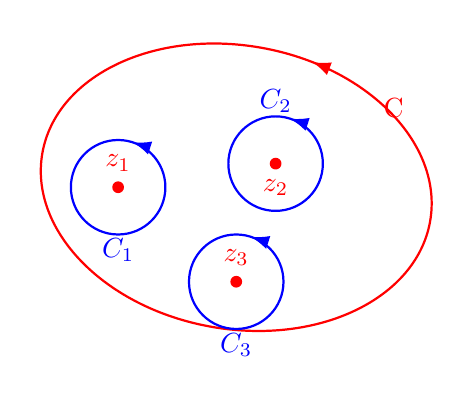
\begin{tikzpicture}[
    >=Latex, % Set default arrow tip style
    curve/.style={thick},    % Base style for curves
    dot/.style={fill=red, circle, inner sep=1.5pt}, % Style for points z1, z2, z3
    labelstyle/.style={}, % Base style for labels
    % Style for placing a CCW arrow (>) on a path
   midarrowL/.style={
        decoration={markings, mark=at position 0.2 with {\arrowreversed{Latex}}},
        postaction={decorate}
    },
    midarrow/.style={
        decoration={markings, mark=at position 0.2 with {\arrow{Latex}}},
        postaction={decorate}
    }
]

    % Define coordinates for points z1, z2, z3
    \coordinate (z1) at (0, 0);
    \coordinate (z2) at (2, 0.3);
    \coordinate (z3) at (1.5, -1.2);

    % Define radius for inner circles
    \def\r{0.6};

    % Define parameters for outer ellipse C (adjust as needed)
    \coordinate (Ccenter) at (1.5, 0); % Approx center
    \def\Cxrad{2.5} % Approx x-radius
    \def\Cyrad{1.8} % Approx y-radius
    \def\Crot{-10}  % Approx rotation

    % Draw Outer Red Ellipse (C) with CCW Arrow
    \draw[curve, red, midarrow] % Arrow near top-left
        (Ccenter) ellipse [x radius=\Cxrad, y radius=\Cyrad, rotate=\Crot];
    \node[red] at (3.5, 1.0) {C}; % Label C

    % Draw Inner Blue Circles C1, C2, C3 with CW Arrows
    % C1
    \draw[curve, blue] (z1) circle (\r); % Draw circle border
    \path[curve, blue, midarrow] (z1) circle (\r); % Add arrow decoration
    \node[blue] at ($(z1)+(-90:\r+0.2)$) {$C_1$}; % Label C1 below
    \node[dot, label={[red]above:$z_1$}] at (z1) {}; % Point z1

    % C2
    \draw[curve, blue] (z2) circle (\r); % Draw circle border
    \path[curve, blue,midarrow] (z2) circle (\r); % Add arrow decoration
    \node[blue] at ($(z2)+(90:\r+0.2)$) {$C_2$}; % Label C2 above
    \node[dot, label={[red]below:$z_2$}] at (z2) {}; % Point z2

    % C3
    \draw[curve, blue] (z3) circle (\r); % Draw circle border
    \path[curve, blue, midarrow] (z3) circle (\r); % Add arrow decoration
    \node[blue] at ($(z3)+(-90:\r+0.2)$) {$C_3$}; % Label C3 below
    \node[dot, label={[red]above:$z_3$}] at (z3) {}; % Point z3

\end{tikzpicture}
\end{document}